En este capítulo se mostrarán las distintas tipologías de pruebas que existen como introducción a las mismas y las que se han realizado tanto en el Backend como en el Frontend para verificar la funcionalidad del sistema añadiendo así calidad a nuestro proyecto.

\newpage

El testing, como concepto general, se basa en investigaciones y técnicas que se encargan de proporcionar información sobre el producto software y de si este cumple con todas las condiciones de calidad para ser llevado a un sistema de producción o de cliente final.

A su vez, como existen distintos tipos de software, existen distintos tipos de pruebas. A continuación, listamos los tipos más genéricos y damos una breve descripción de para que sirven.

\begin{itemize}
    \item Pruebas unitarias: se basa en comprobar la veracidad o funcionamiento correcto de un trozo de código, generalmente una función o método de un objeto.
    \item Pruebas de integración: se realizan siempre a posteriori de las pruebas unitarias y se basa justamente en probar en conjunto lo probado en las pruebas unitarias para comprobar que la integración de esas funcionalidades no da ningún error.
    \item Pruebas de humo: son pruebas rápidas, generalmente manuales, que se encarga de comprobar el flujo principal del software y algunos casos secundarios, pero sin profundizar en ellos.
    \item Pruebas alpha: son pruebas que se hacen durante el desarrollo del software y se encargan de verificar que el producto software que se está desarrollando, es útil y válido para el cliente.
    \item Pruebas beta: son pruebas que se hacen cuando el desarrollo está terminado y se hacen en un entorno semireal o de semiproducción.
    \item Pruebas de aceptación: estas pruebas se realizan cuando la generación de la release del producto software está próxima y se encarga de verificar que se cumplen todos los requisitos funcionales. Se alternan pruebas automáticas y manuales.
    \item Pruebas de regresión: estas pruebas se basan en buscar errores, en lugar de buscar una correcta ejecución del software. Son bastantes últiles a la hora de detectar situaciones limite no contempladas anteriormente.
    \item Pruebas de compatibilidad: se basa en probar el sistema de distintos entorno para comprobar su correcto funcionamiento. Esto no es más que, ejecutar el software en distintos sistemas operativos para ver que ocurre.
    \item Pruebas de usabilidad: estas pruebas suelen ser manuales y se basan en que los distintos usuarios para lo que está orientado el producto software interactúen con dicho programa y detecten las carencias que tenga en materia de usar el propio software.
    \item Pruebas de rendimiento: estas pruebas se basan en ejecutar el software en distintas máquinas con variedad de recursos hardware para ver como se comporta. Si el software solo puede ejecutarse con una especificación hardware en concreto, no se considera de inmediato que el software este mal, si no que eso hay que contrastarlo con las especificaciones hardware del sistema de producción.
    \item Pruebas de escalabilidad: estas pruebas suelene ser automáticas y se basan en aplicar distinta carga de datos de entrada al software y ver como es capaz de escalar según la demanda y sus recursos software asignados. Este tipo de pruebas esta íntimamente ligadas con las pruebas de carga.
\end{itemize}

Pero, según el software, se aplican unas pruebas u otras. En el contexto de los sistemas distribuidos, se puede dividir en 2 grupos:

\begin{itemize}
    \item Pruebas funcionales: son pruebas de caja negra que se centra en que dada una precondición, se cumple una postcondición en un tiempo determinado. Su función principal es comprobar si el producto tiene la calidad suficiente para entrar en producción.
    \item Pruebas no funcionales: son pruebas dedicadas a comprobar detalles que no estén intimamente ligados con el uso final del software.
\end{itemize}

Así pues, pasaremos a definir que tipos de test se han realizado en los 2 bloques principales.

\section{Backend}
En el Backend, las principales pruebas han sido manuales. La única prueba automática se ha realizado ha sido la concerniente a la creación, login y eliminación de un usuario.

Es decir, se ha hecho una prueba automátizada para probar todo el ciclo de vida de un usuario.

Esta prueba se ha realizado de forma automatizada, ya que, prueba uno de los aspectos más importantes de la aplicación. Es decir, la seguridad de acceso al sistema.

Esta prueba ha sido realizada con MochaJS \cite{mochajs}.

Por lo demás, se ha probado todo de forma manual e integrado con el Frontend. El motivo de no haber hecho más pruebas automatizadas ha sido el tiempo y la no necesidad de ser exhaustivo en este aspecto con un proyecto de esta magnitud.

A continuación, en la Figura 7.1, se muestra el resultado de los test en el Backend.

\begin{figure}[H]
    \centering
    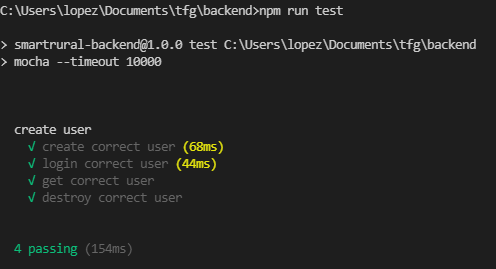
\includegraphics[width=0.7\linewidth]{images/test/test user backend.png}
    \caption{npm run test}
\end{figure}

\section{Frontend}
En el Frontend, todas las pruebas realizadas han sido manuales integradas con el Backend. La única prueba realizada de forma automática ha sido una prueba generica donde se comprueba que la aplicación base se renderiza de forma correcta. Esta prueba ha sido realizada con Jest \cite{jest}. En la Figura 7.2 se muestra el resultado de los tests.

\begin{figure}[H]
    \centering
    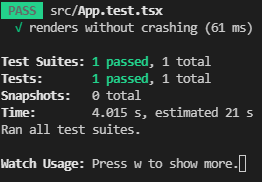
\includegraphics[width=0.7\linewidth]{images/test/test app frontend.png}
    \caption{npm run test}
\end{figure}

Por lo demás, todo ha sido probado con distintas pruebas manuales en integración con el Backend, a la hora de comprobar si obtenia la información de forma correcta y rápida.